\documentclass[fleqn,12pt]{wlscirep}
% * <jpschoen@gmail.com> 2018-03-07T16:08:10.834Z:
%
% ^.
\usepackage{natbib}
\usepackage{geometry}
\usepackage{pdflscape}
\usepackage{longtable}
%\newgeometry{margin=1cm} % modify this if you need even more space
\usepackage[final]{pdfpages}
\setboolean{@twoside}{false}
\linespread{1}
\usepackage{booktabs,tabularx}
\usepackage[input-decimal-markers=.]{siunitx}
\usepackage{lipsum}




\title{\centering{Chapter 48 Outline\\
%\vspace{1cm}
\large{Network Modeling: Estimation, Inference, Comparison, and Selection}
%\vspace{1cm}
}}
{\centering
\author[1]{John P. Schoeneman}
\author[1]{Bruce A.  Desmarais}
\affil[1]{Penn State, Political Science, University Park, Pond Lab}
}
\begin{document}

\flushbottom
\maketitle{}
%\keywords{Keyword1, Keyword2, Keyword3} 
\vspace{-1.5cm}
\noindent {\bf Introduction:} 



\section{Introduction}

Do states go to war with the enemies of their enemies? Which international trade relationships are most likely to break down over the next decade? What would happen to the  Statistical inference with network data permits researchers to test hypotheses about network generation, predict network structure, and simulate networks from probabilistic models. How would the world system of military alliances rewire if the United States were to exit the North Atlantic Treaty Organization? What these questions have in common is that they  address systems of international relationships (conflict, trade, and alliances)---systems that can be represented as networks in which the states constitute the nodes, and the relationships constitute the edges between nodes. Inferential network analysis represents a methodological class that can be drawn upon to answer questions like these. Most statistical models used in the social sciences rely on the assumption that the observations in a dataset (or at least clusters of observation) are drawn independently from a common data generating process.  However, when analyzing networks it is often inappropriate to assume that observations are independent \citep{harris2013communication,hafner2009network}. Indeed, the network analyst is often interested in studying the ways in which observations depend upon each other \citep{ogburn2018challenges} (e.g., do friends influence each others' choices to vote \citep{bond201261}, do legislators reciprocate support for legislation \citep{kirkland2014partisanship}). 

Many, perhaps even most, of the empirical phenomena of interest to scholars of international relations can be represented as international networks. Paired with the availability of accessible software implementations, the conceptual appropriateness of inferential network analysis in international relations has led to widespread application over the last 10--15 years. Networks that have been studied through the use of inferential network analysis include, but are not limited to, trade \citep{ward2007persistent,agiolo2014does,chu2010homogenization,chyzh2016dangerous}, conflict \citep{ward2007disputes,cranmer2011inferential,gallop2016endogenous,dorff2013networks}, alliances \citep{cranmer2012complex, }, transnational terrorism \citep{desmarais2013forecasting,asal2016friends,metternich2013antigovernment,bush2015measuring}, sanctioning \citep{cranmer2014reciprocity,dorff2017states}, IGOs \citep{cao2012global,dorussen2008intergovernmental,lupu2017networked} [CITES] and NGOs \citep{atouba2015international} [CITES]. This research has led to several innovative findings. For example, [SOMETHING FROM KINNE's WORK], latent network structure can be used to forecast the evolution of civil conflict [CITE SHAHRYAR's STUFF], [CITE A FINDING FROM OLGA's WORK]. Inferential network analysis is a valuable piece in the IR scholar's toolkit.
 
Methods for inferential network analysis come primarily in the form of probabilistic models for networks, which are fit to data using common estimation frameworks (e.g., maximum likelihood estimation, Bayesian inference). Inferential network analysis is now far too broad of a methodological area to effectively review all of the models in any detail. In what follows we will review three modeling approaches in detail. These include the exponential random graph model (ERGM) \citep{cranmer2011inferential}, the latent space model (LSM) \citep{dorff2016latent},  and the stochastic block model (SBM) \citep{latouche2011overlapping}. The first model, which we refer to as the latent space model (LSM), is a class of models in which each node is attributed with a position in a latent space of features. The second model, the exponential random graph model (ERGM) is a model that can be customized to represent networks with any quantifiable characteristic (e.g., a high number of reciprocated ties, a strong degree of clustering).  The third model we discuss in detail is the stochastic blockmodel (SBM). The first two models, LSM and ERGM, are commonly used in international relations. The SBM, however, has seen little use in IR. We make the case that the SMB should be used in political science as an alternative to ERGM and SBM. After presenting a review of these three models, we provide a brief overview of several approaches that we did not review in detail, but of which IR scholars should be aware. After reviewing these models we present an application in which we replicate the analyses from  using each of these models and focus in particular on the application of SBM, since SBM is new in IR.


In this chapter we will review three of the most popular statistical models that have been developed to analyze network data, along with their extensions. These include the exponential random graph model (ERGM) \citep{cranmer2011inferential}, the latent space model (LSM) \citep{dorff2016latent},  and the stochastic block model (SBM) \citep{latouche2011overlapping}. We will review the application of each method to networks in which ties are binary (e.g., are two legislators on at least one committee together), count (e.g., on how many committees do two legislators both serve), and continuous (e.g., how much time do two legislators spend together in committee meetings each week). The complexity and analytical intractability of the mathematical forms of these models render exact approaches to likelihood maximization infeasible. As such, estimation in these models proceeds by sampling from a Bayesian posterior and/or approximate methods of maximum likelihood \citep{raftery2012fast,van2009framework,nowicki2001estimation}. We will review these estimation methods, and how they are applied to the ERGM, LSM, and SBM.  This chapter will be divided into three sections. In the first section we will give an overview of the most common models used in network analysis. In the second section we will discuss the approaches to estimation that are commonly used with these models. In the last section we will provide an application of all three models, .

\section{Model description}

The three models we review in detail, the LSM, ERGM, and SBM share a common starting point in the case of dichotomous edges (i.e., the edge does or does not exist). Consider a research problem in which the researcher is interested in using covariates that can be measured on the directed pair $(i,j)$, where $i$ is the index of the potential sender of an edge, and $j$ is the index of the potential receiver of the edge, to model whether the edge $(i,j)$ exists. Denote the edge indicator $y_{i,j} = 1$  if there is an edge from node $i$ to node $j$, and 0 otherwise. Let $x_{i,j}$ be a covariate that can be measured on the directed dyad (e.g., if the nodes are states, the distance between their capital cities), or mapped to the dyad (e.g., $x_{i,j}$ is the GDP of the sender state, $i$). A standard approach to modeling the dyadic variable $y$ as a function of $x$ would be to estimate a logistic regression in which $y$ is the dependent variable and $x$ is the independent variable. The LSM, ERGM, and SBM all reduce to a logistic regression in which edge indicators are regressed on measured covariates in the case where the network components of the respective models do not contribute to the fit of the model [CITES]. In other words, logistic regression is a special case of LSM, ERGM, and SBM. 

In the case of each model, network structure is layered on top of the simple logistic regression [PROBIT FOR AMEN?]. The particular form of network structure added varies across the models. In the LSM, each node is represented by some number of continuous-valued features (e.g., coordinates in a Euclidean space), and the probability of a tie is given by some function of the features (e.g., the Euclidean distance between nodes). We refer to the network structure incorporated in the LSM framework as `selection', since the function defined on the latent feature serves as a partner selection function for nodes in the network. The network component under ERGM is designed to capture the prevalence of subnetworks that are theoretically interesting or otherwise distinct. Examples of these subnetworks include triangles (i.e., triples of nodes $(i,j.k)$ in which there is an edge connecting each pair of nodes), and mutual dyads (i.e., dyads in which there is an edge from $i$ to $j$ and from $j$ to $i$). In the ERGM, subnetwork prevalence is controlled through the incorporation of dependence among the edges. For example, if a network is modeled to have a relatively high number of mutual dyads, the formation of an edge from $i$ to $j$ increases the likelihood that an edge will form from $j$ to $i$. Since the basic building blocks of the network component of the ERGM reflect different forms of dependence, we refer to the network structure in the ERGM as `dependence'. The network structure of the SBM is build on a common interest in identifying the communities, clusters, or groups that define the main blocks of ties in the networks. Under the SBM's network structure, the blocks of which two nodes are members determines whether those two nodes will form an edge. Since the network component of the SBM is focused on segmenting the nodes into a set of groups, we refer to the network structure in the SBM as segmentation.

\subsection{Latent space modeling of networks}
The notion of selection is deeply rooted in the international relations literature. The likelihood that one state initiates a militarized conflict against another state has been found to be a function of both the sender and receiver states' level of democratization [CITES], the ratio of the two states' military capabilities scores [CITE], and the geographic distance between the two states [CITES]. The probability of conflict initiation is given by a combination of a variety of functions applied to a variety of states' features. The LSM reflects this very structure---the probability of a tie depending on a combination of functions of node features---with exception being that the features inferred in the LSM are latent. That is, given one or more functions according to which the latent features affect the probability of an edge,  in the LSM the nodes' feature values are inferred to be those that best explain the pattern of edges observed in the data.

\subsection{The exponential random graph model}

Theories of dependence in international relations have been developing rapidly in recent years. Example findings include that there is a strong tendency towards rapid retaliation in the issuance of international economic sanctions, SOMETHING FROM A SAOM PAPER, SOMETHING FROM ANOTHER ERGM PAPER.  The ERGM opens up a new class of hypotheses that can be tested relative to regression models. In addition to studying how covariates effect the absence/presence of edges, the ERGM permits researchers to test hypotheses about how the edges effect each other (e.g., is the enemy of an enemy a friend)? The key components in using an ERGM are to develop hypotheses regarding the ways in which edges depend on each other, and conceptualize these dependencies in terms of subnetwork structures such as dyads and triads.

\subsection{The stochastic blockmodel}

Concepts in international relations related to system polarity [CITES], [CONCEPT FROM ELIZABETH AND SKYLER], fall within the orbit of the SBM formulation. Under the SBM there is a finite number of node types or `blocks', and each block is defined by the probabilities according to which nodes within the block form ties with each other, and with nodes in other blocks. If there are $n$ nodes in the network, the SBM reduces the complexity of interactions among those $n$  nodes, to interactions among and within a set of $b$ blocks, where $b$ is typically much smaller than $n$. 


Segmentation SBM is common elsewhere, and should be used more in polisci

\subsection{Additional methods in brief}

The LSM, ERGM, and SBM reflect the core components

\section{Application of ERGM, LSM, and SBM}

{\bf [John]}: [Background summary of Wojcik paper]

For the application we replicate a recent study on the determining factors for when actors form connections in Brazilian legislative networks. The author argues that despite high levels of personalism in Latin American politics, political parties are equally effective in determining actor behavior, indicating that there are higher levels of party discipline than previously thought.


{\bf [John]}: [summary of replication/extension]

In addition to replicating the ERGM models in the article, we also fit the three models using latent space models and stochastic block models. We use the R software package \texttt{ergm} to replicate the ERGM models, \texttt{latentnet} for the LSMs, and \texttt{CIDnetworks} for the SBMs.  We fit models using 2 to 5 blocks for the SBMs. In general we find that results from all the models match the general conclusions of the paper. Below I explain the data from the study, the model specifications, and the results in more detail.

\subsection{Data from wojcik2017legislative}

{\bf [John]}: [One paragraph reviewing how wojcik gathered dependent variable network] 

interactive digital Survey by office managers for Brazilian equivalent of House of Representatives in US. for three different types of connections: communication on legislative issues, socialize about non legislative issues, and information to resolve questions about legislative proposals/procedures.
Also collected biographic info on those that complete the survey to look for any identifiable biases.  Compared traits of sample to that of the entire Congress and found no identifiable difference.

25\% response rate. Filled in missing data with pen and paper survey from 2013.

{\bf [John]}: [One paragraph providing descriptive statistics on the dependent variable network, perhaps include a network plot]

\begin{table}[!htbp] \centering
  \caption{Summary Statistics: DVs}
  \label{}
\begin{tabular}{@{\extracolsep{5pt}} lccccc}
\\[-1.8ex]\hline
\hline \\[-1.8ex]
Network & Measurement & Global Value & Mean & s.d. & Max  \\
\hline \\[-1.8ex]
Communication& Edge Density & $0.008$ & $NA$ & $NA$& $NA$\\
Communication& Degree Distribution & $NA$ & $3.307$ & $3.020$  & $18.000$\\
Communication& Centrality & $0.072$ & $204.588$ & $448.319$  &$3009.852$ \\
Communication& Reciprocity  & $0.255$ & $NA$ & $NA$ &$NA$\\
Communication& Transitivity  & $0.108$ & $NA$ & $NA$ &$NA$\\
\hline \\[-1.8ex]

Social& Edge Density & $0.006$ & $NA$ & $NA$ &$NA$\\
Social& Degree Distribution & $NA$ & $2.482$ & $2.254$  & $11.000$\\
Social& Centrality & $0.025$ & $103.633$ & $222.925$  & $1009.333$\\
Social& Reciprocity  & $0.203$ & $NA$ & $NA$ &$NA$\\
Social& Transitivity  & $0.119$ & $NA$ & $NA$ &$NA$\\
\hline \\[-1.8ex]

Info Exchange& Edge Density & $0.009$ & $NA$ & $NA$ &$NA$\\
Info Exchange& Degree Distribution & $NA$ & $$-$0.348$ & $$-$0.391$  & $6.000$\\
Info Exchange& Centrality & $0.001$ & $0.880$ & $1.930$ & $10.000$\\
Info Exchange& Reciprocity  & $0.157$ & $NA$ & $NA$&$NA$\\
Info Exchange& Transitivity  & $ 0.135$ & $NA$ & $NA$&$NA$\\
\\[-1.8ex]\hline
\hline \\[-1.8ex]
\end{tabular}
\end{table}


 {\bf [John]}: [One paragraph reviewing the independent variables in the analysis, perhaps include a table of descriptive data]

\begin{table}[!htbp] \centering
  \caption{Summary Statistics: IVs}
  \label{}
\begin{tabular}{@{\extracolsep{5pt}} lccc}
\\[-1.8ex]\hline
\hline \\[-1.8ex]
 &  \multicolumn{3}{c}{Proportion} \\
\hline \\[-1.8ex]
Variable & Communication & Social & Info Exchange\\
\hline \\[-1.8ex]

Same Education Level  & $71\%$ & $70\%$ & $74\%$\\
Same Floor  & $10\%$ & $10\%$ & $12\%$\\
Both Leadership & $6\%$ & $7\%$ & $6\%$\\
Both non-Leadership & $10\%$ & $10\%8$ & $14\%$\\
Same State  & $10\%$ & $70\%$ & $74\%$\\
Same Party & $46\%$ & $10\%$ & $12\%$\\
\hline \\[-1.8ex]
 &  \multicolumn{3}{c}{Average} \\
\hline \\[-1.8ex]
$\Delta$ Age & $12$ & $12$ & $13$\\
\\[-1.8ex]\hline
\hline \\[-1.8ex]
\end{tabular}

\end{table}





Main hypotheses: 
Same political party: Parties actively work to form ties within and among members to counter the individualistic tendencies of politicians to increase their own electoral share/power at the expense of the party. The network then creates trust and cohesion among the actors, while also facilitating monitoring.Author expects this will the the stronger driver of the tie formation, rather than individual traits. 

Secondary hypotheses is that similar individual traits drive network ties. 

both are in leadership positions, 
neither are in leadership positions 

absolute difference in age: similar age will drive politicians to form connections based on shared experiences. 

Same state: proportional voting system in Brazil means that coordination among members in the same states is necessary to exchange information about what the local needs are. 

Same education level: (pre-high school, high school, college, and above college): likely to have similar knowledge and social class, which increases the change of network ties. 

Same floor: floor of the building they work on: creates opportunity for interaction.


\subsection{Replication design}

 {\bf [John]}: [One paragraph reviewing the model specification in the original paper, explaining the transitive ties term ]
 
The models is specified in the article to include a intercept term, the exogenous covariates, and a term for transitive ties, or the change in the likelihood of a tie between two nodes given the presence of a two-path or a triad closure. A two-path between nodes $i$ and $j$ is defined as  node $i$ having a directed edge path to node $k$ and node $k$ having a directed edge to node $j$, thus you can find a connection between the nodes with only two edges.
 

 {\bf [John]}: [One paragraph describing how we extend the application to use both the LSM and the SBM]

For the LSM model, the specification is the same except it does not include the include a transitive ties term. This is because the model does not have network statistics as an ERGM model does, but instead we specify the latent space effects that models higher order dependences. For our extensions we use the euclidean distance model term that is equal to the negative euclidean distance between actors in the unobserved social space. We estimated the term along two dimensions and across two blocks. The SBM does not include a constant term as the block or group effect takes the place of the intercept term. It also does not have network terms like transitive ties as it accounts for dependencies using the latent space along a multinomial distribution to determine block membership for the nodes. 


\subsection{Results}

 {\bf [John]}: [1--2 paragraphs discussing covariate results that are consistent and/or different across the ERGM LSM, and SBM. ]


 {\bf [John]}: [1--2 paragraphs discussing the latent structure in the LSM and SBM (i.e., visuals of the LSM estimates, distribution of nodes by blocks in the SBMs) ]

% Table created by stargazer v.5.2.2 by Marek Hlavac, Harvard University. E-mail: hlavac at fas.harvard.edu
% Date and time: Mon, Dec 17, 2018 - 20:18:54
\begin{table}
\begin{center}
\begin{tabular}{l c c c }
\hline
 & Model 1 & Model 2 & Model 3 \\
\hline
 edges & $-$5.670$^{***}$ & $-$6.070$^{***}$ & $-$5.742$^{***}$ \\ 
  & (0.162) & (0.185) & (0.445) \\ 
  & & & \\ 
 absdiff.age & $-$0.021$^{***}$ & $-$0.024$^{***}$ & $-$0.063$^{***}$ \\ 
  & (0.007) & (0.008) & (0.022) \\ 
  & & & \\ 
 nodematch.education & 0.164 & 0.161 & 0.600$^{*}$ \\ 
  & (0.125) & (0.144) & (0.334) \\ 
  & & & \\ 
 nodematch.floor & 0.756$^{***}$ & 1.373$^{***}$ & 0.794$^{**}$ \\ 
  & (0.153) & (0.141) & (0.390) \\ 
  & & & \\ 
 nodematch.leadership.FALSE & $-$0.655$^{***}$ & $-$0.241$^{*}$ & $-$0.805$^{**}$ \\ 
  & (0.125) & (0.139) & (0.337) \\ 
  & & & \\ 
 nodematch.leadership. & 0.534$^{***}$ & 0.473$^{**}$ & 0.837$^{**}$ \\ 
  & (0.164) & (0.206) & (0.396) \\ 
  & & & \\ 
 nodematch.UF & 2.121$^{***}$ & 2.106$^{***}$ & 0.989$^{**}$ \\ 
  & (0.124) & (0.140) & (0.431) \\ 
  & & & \\ 
 nodematch.party & 2.319$^{***}$ & 2.051$^{***}$ & 2.958$^{***}$ \\ 
  & (0.123) & (0.135) & (0.343) \\ 
  & & & \\ 
 transitiveties & 0.661$^{***}$ & 0.901$^{***}$ & 0.568 \\ 
  & (0.123) & (0.139) & (0.399) \\ 
  & & & \\ 
\hline \\[-1.8ex] 
Akaike Inf. Crit. & 3,056.153 & 2,281.901 & 466.732 \\ 
Bayesian Inf. Crit. & 3,133.387 & 2,358.395 & 526.326 \\ 
\hline
\multicolumn{4}{l}{\scriptsize{Note: {$^{*}$p$<$0.1; $^{**}$p$<$0.05; $^{***}$p$<$0.01}}}
\end{tabular}
\caption{ERGM results}
\label{table:coefficients}
\end{center}
\end{table}



\begin{table}
\begin{center}
\begin{tabular}{l c c c }
\hline
 & Model 1 & Model 2 & Model 3 \\
\hline
edges                      & $-3.42^{*}$       & $-3.13^{*}$       & $-3.16^{*}$       \\
                           & $[-3.66;\ -3.21]$ & $[-3.64;\ -2.65]$ & $[-4.20;\ -2.08]$ \\
absdiff.age                & $-0.02^{*}$       & $-0.04^{*}$       & $-0.07^{*}$       \\
                           & $[-0.03;\ -0.02]$ & $[-0.06;\ -0.03]$ & $[-0.11;\ -0.03]$ \\
nodematch.education        & $0.62^{*}$        & $0.29$            & $0.95^{*}$        \\
                           & $[0.61;\ 0.62]$   & $[-0.10;\ 0.72]$  & $[0.02;\ 1.82]$   \\
nodematch.floor            & $1.04^{*}$        & $1.65^{*}$        & $1.19^{*}$        \\
                           & $[1.02;\ 1.06]$   & $[1.61;\ 1.71]$   & $[0.25;\ 2.09]$   \\
nodematch.leadership.FALSE & $-0.80^{*}$       & $-0.19^{*}$       & $-0.80^{*}$       \\
                           & $[-1.08;\ -0.61]$ & $[-0.19;\ -0.19]$ & $[-1.65;\ -0.10]$ \\
nodematch.leadership.TRUE  & $1.03^{*}$        & $0.57^{*}$        & $0.29^{*}$        \\
                           & $[0.95;\ 1.08]$   & $[0.51;\ 0.60]$   & $[0.10;\ 0.44]$   \\
nodematch.UF               & $2.79^{*}$        & $3.07^{*}$        & $1.44^{*}$        \\
                           & $[2.79;\ 2.79]$   & $[2.99;\ 3.13]$   & $[1.14;\ 1.71]$   \\
nodematch.party            & $2.99^{*}$        & $2.58^{*}$        & $3.40^{*}$        \\
                           & $[2.99;\ 3.00]$   & $[2.58;\ 2.58]$   & $[2.60;\ 4.17]$   \\
\hline
BIC (Overall)              & 3598.75           & 2936.78           & 750.59            \\
BIC (Likelihood)           & 2514.75           & 1839.25           & 385.66            \\
BIC (Latent Positions)     & 1084.00           & 1097.53           & 364.93            \\
\hline
\multicolumn{4}{l}{\scriptsize{$^*$ 0 outside the confidence interval}}
\end{tabular}
\caption{LSM results}
\label{table:coefficients}
\end{center}
\end{table}


\clearpage
\begin{longtable}[!h]{c@{\hskip 0cm}c}
Age, Absolute Difference \\
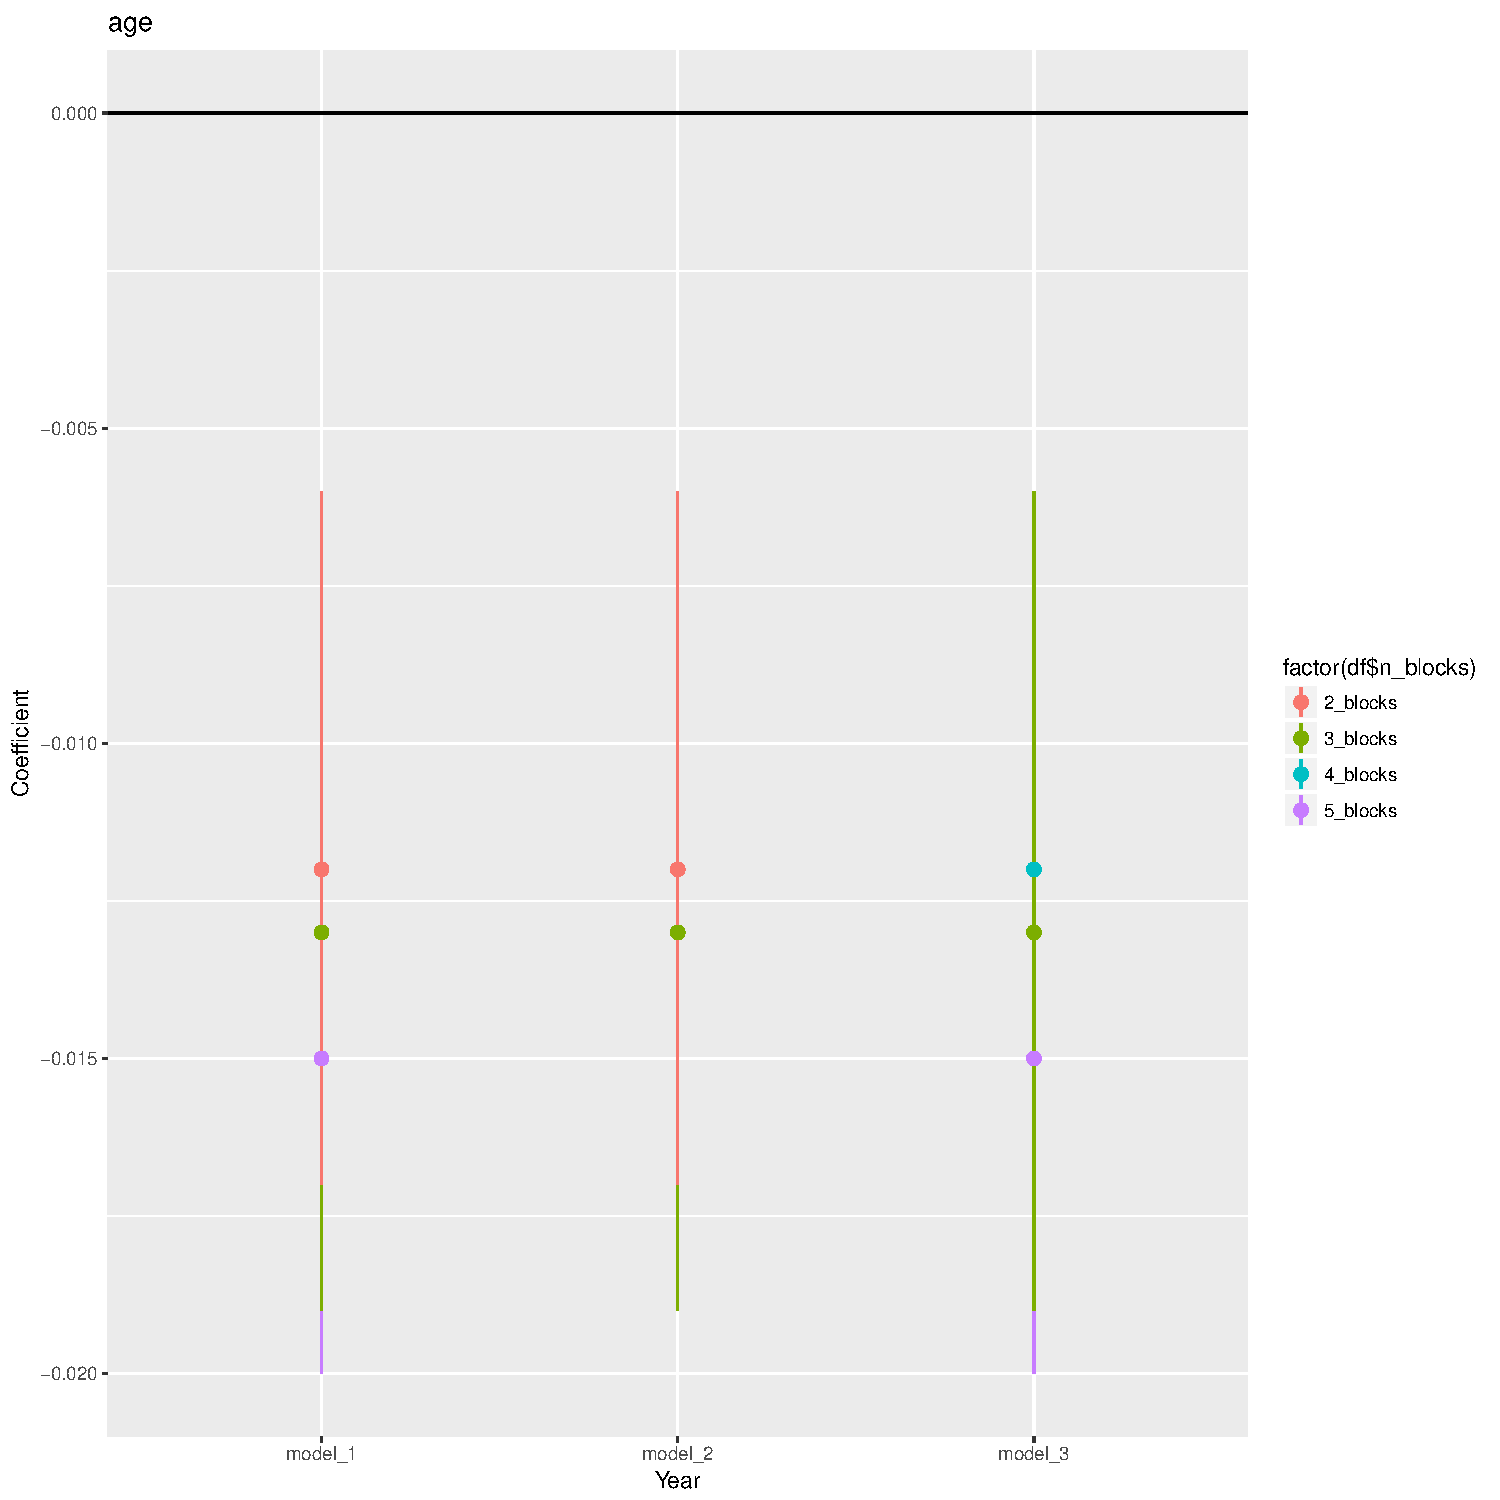
\includegraphics[height=.75\textheight, clip=true, trim=.5cm .5cm 0cm .6cm]{figures/rl_plots1/age.pdf} \\
\caption{\label{fig:SBM_plot_pref} SBM covariate plot. Results from models for which DIC could not be calculated were discarded.}
\end{longtable}

\clearpage
\begin{longtable}[!h]{c@{\hskip 0cm}c}
Education, node match \\
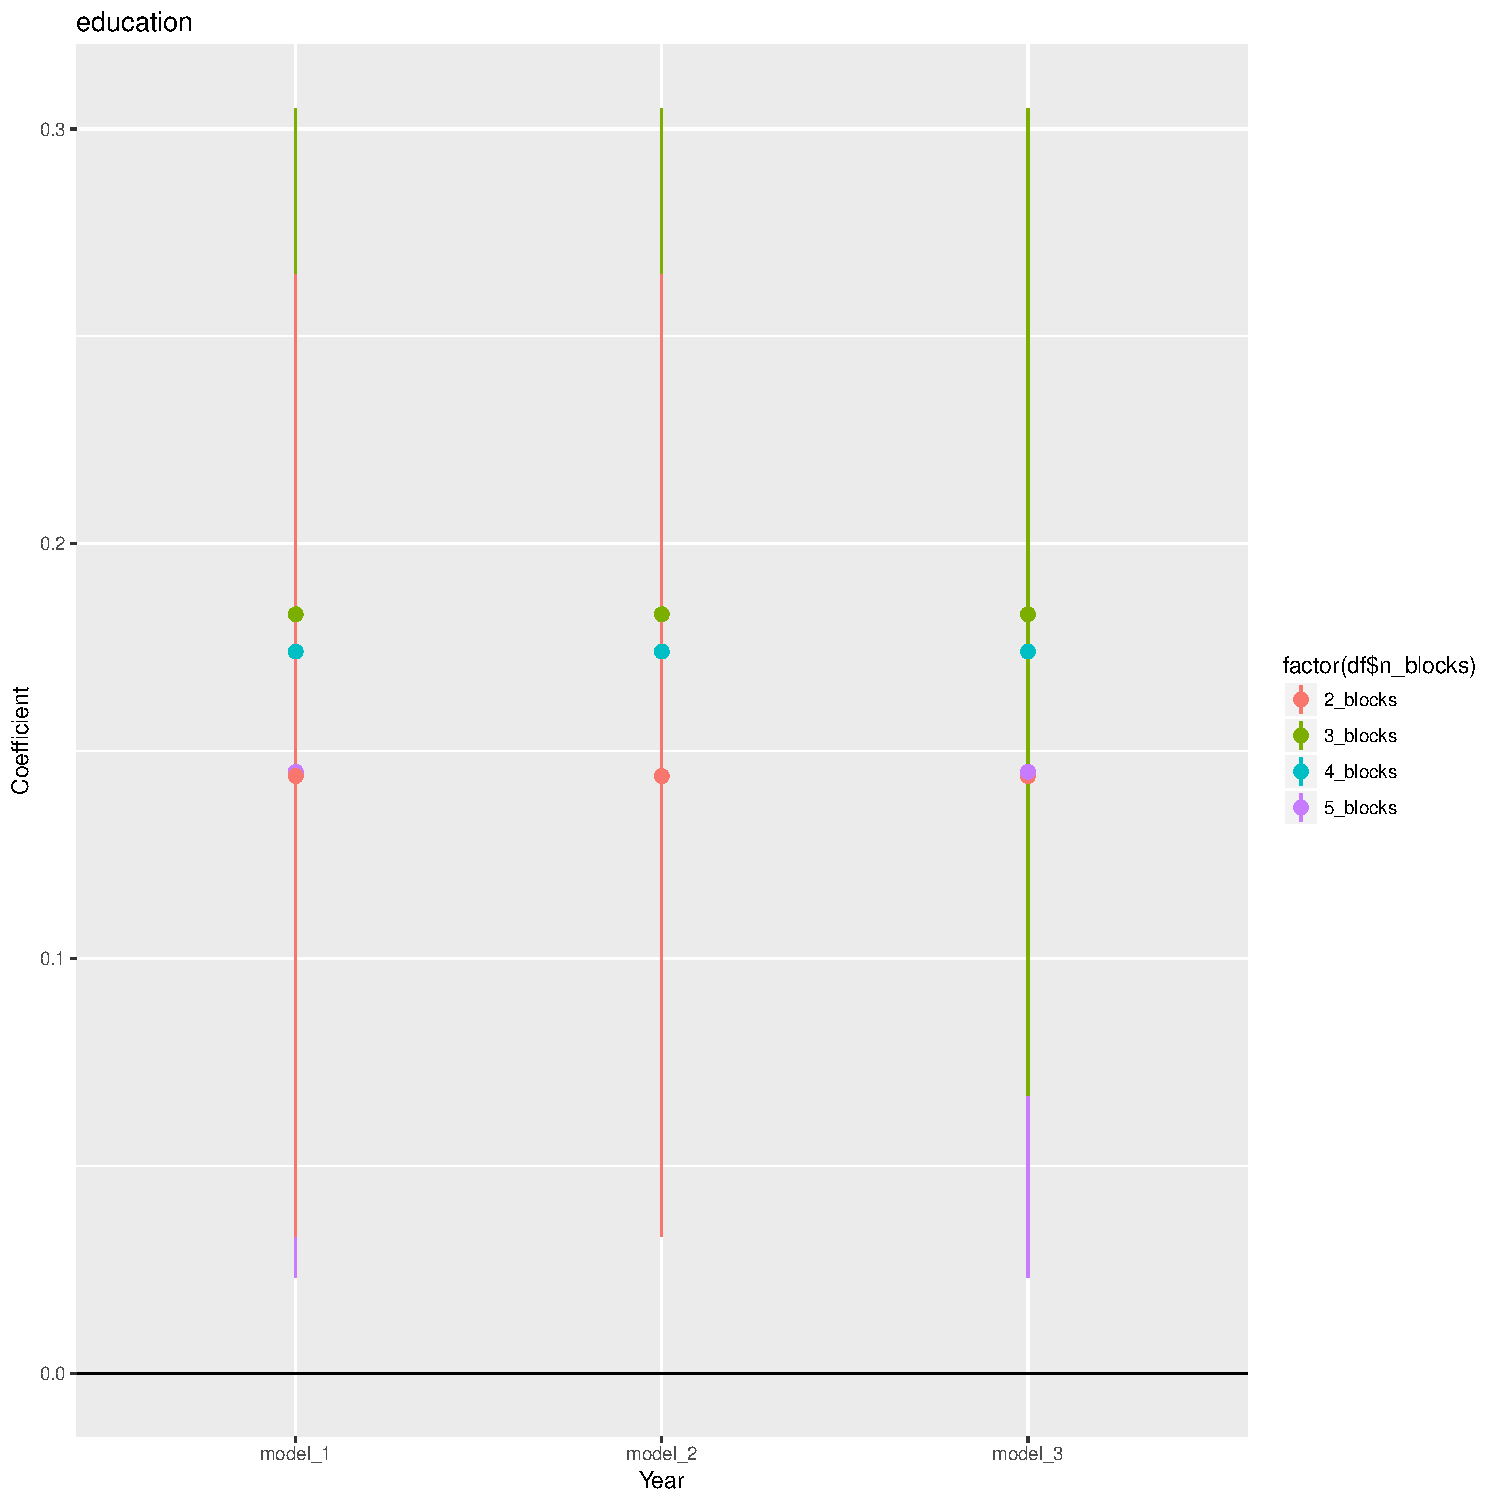
\includegraphics[height=.75\textheight, clip=true, trim=.5cm .5cm 0cm .6cm]{figures/rl_plots1/education.pdf}   \\
\caption{\label{fig:SBM_plot_gov} SBM covariate plot. Results from models for which DIC could not be calculated were discarded.}
\end{longtable}

\clearpage
\begin{longtable}[!h]{c@{\hskip 0cm}c}
Office floor, nodematch \\
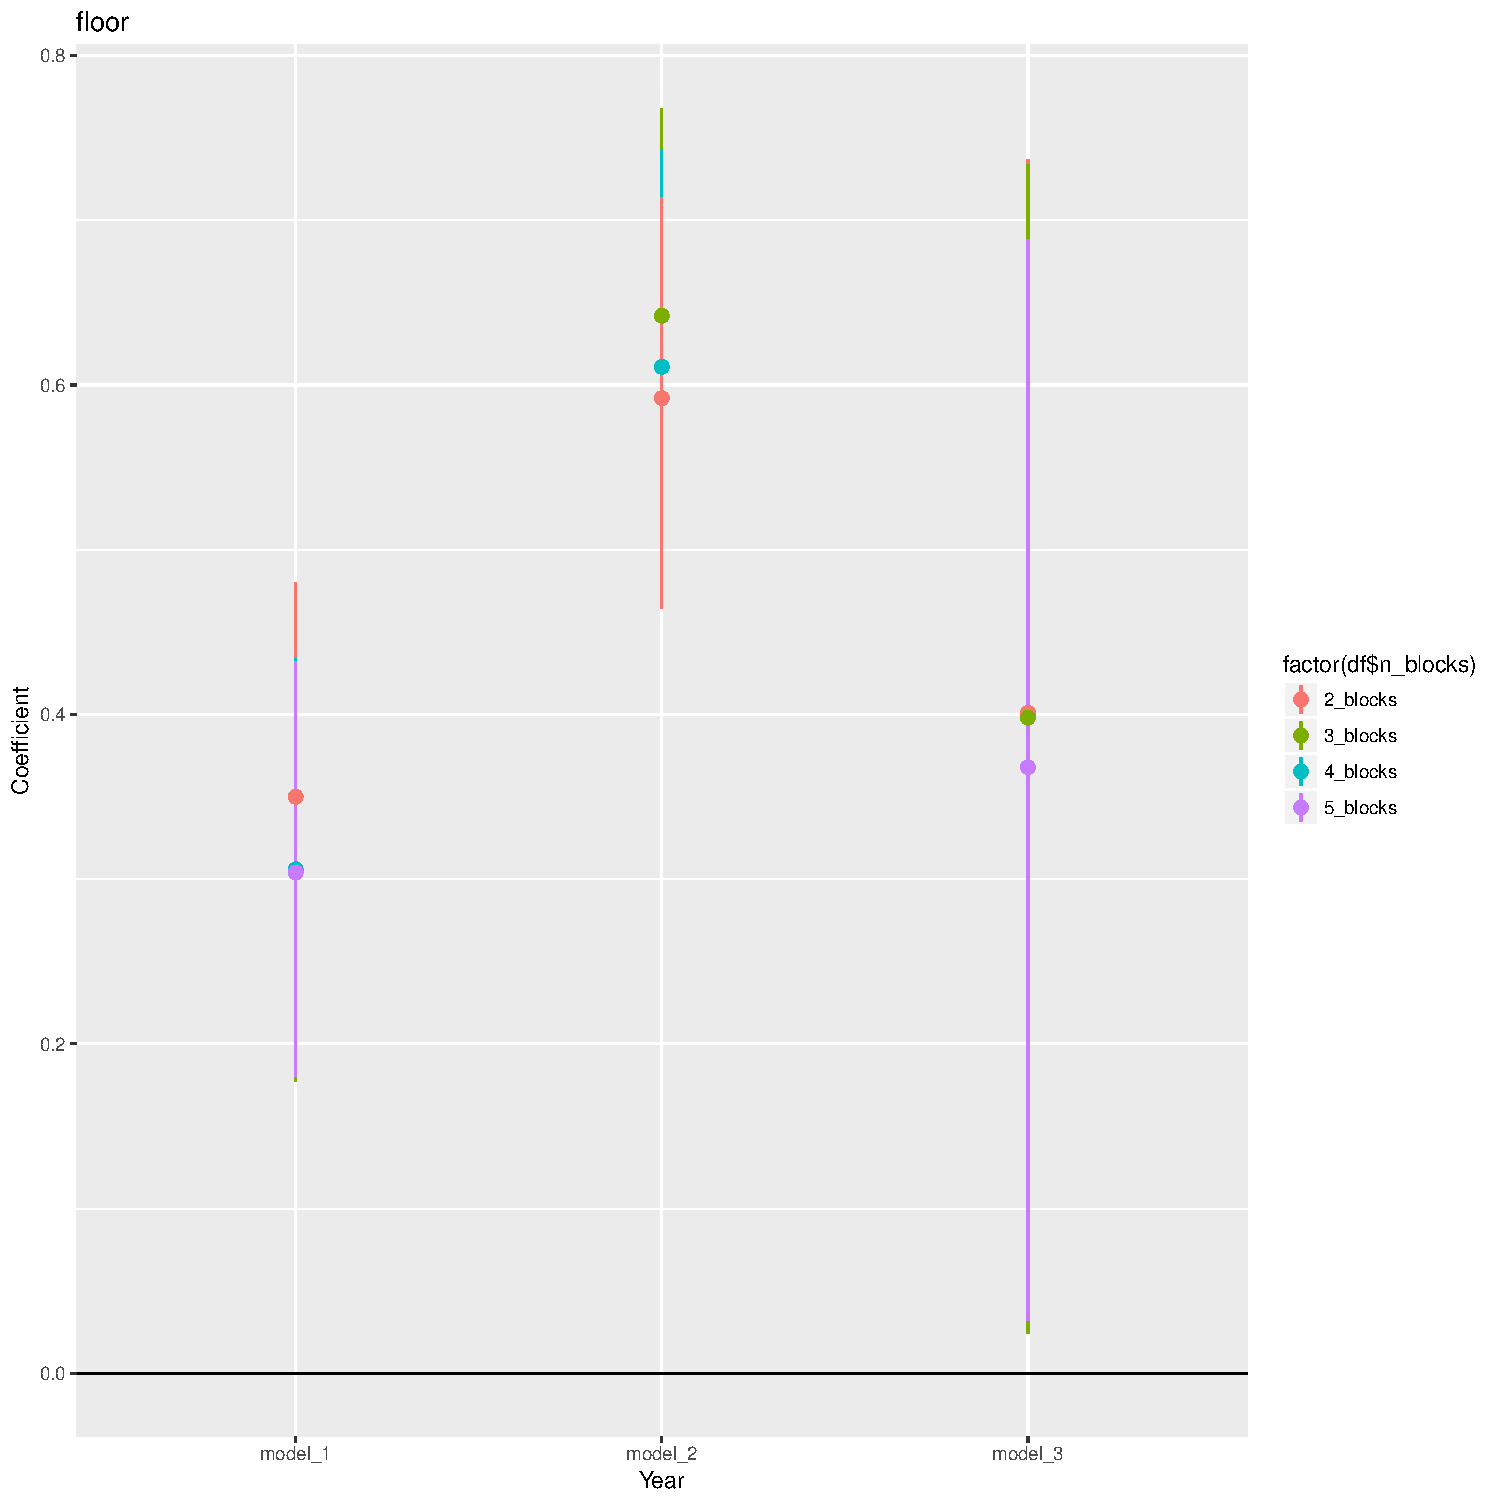
\includegraphics[height=.75\textheight, clip=true, trim=.5cm .5cm 0cm .6cm]{figures/rl_plots1/floor.pdf}   \\
\caption{\label{fig:SBM_plot_sci} SBM covariate plot. Results from models for which DIC could not be calculated were discarded.}
\end{longtable}

\clearpage
\begin{longtable}[!h]{c@{\hskip 0cm}c}
Not Leadership, nodematch \\
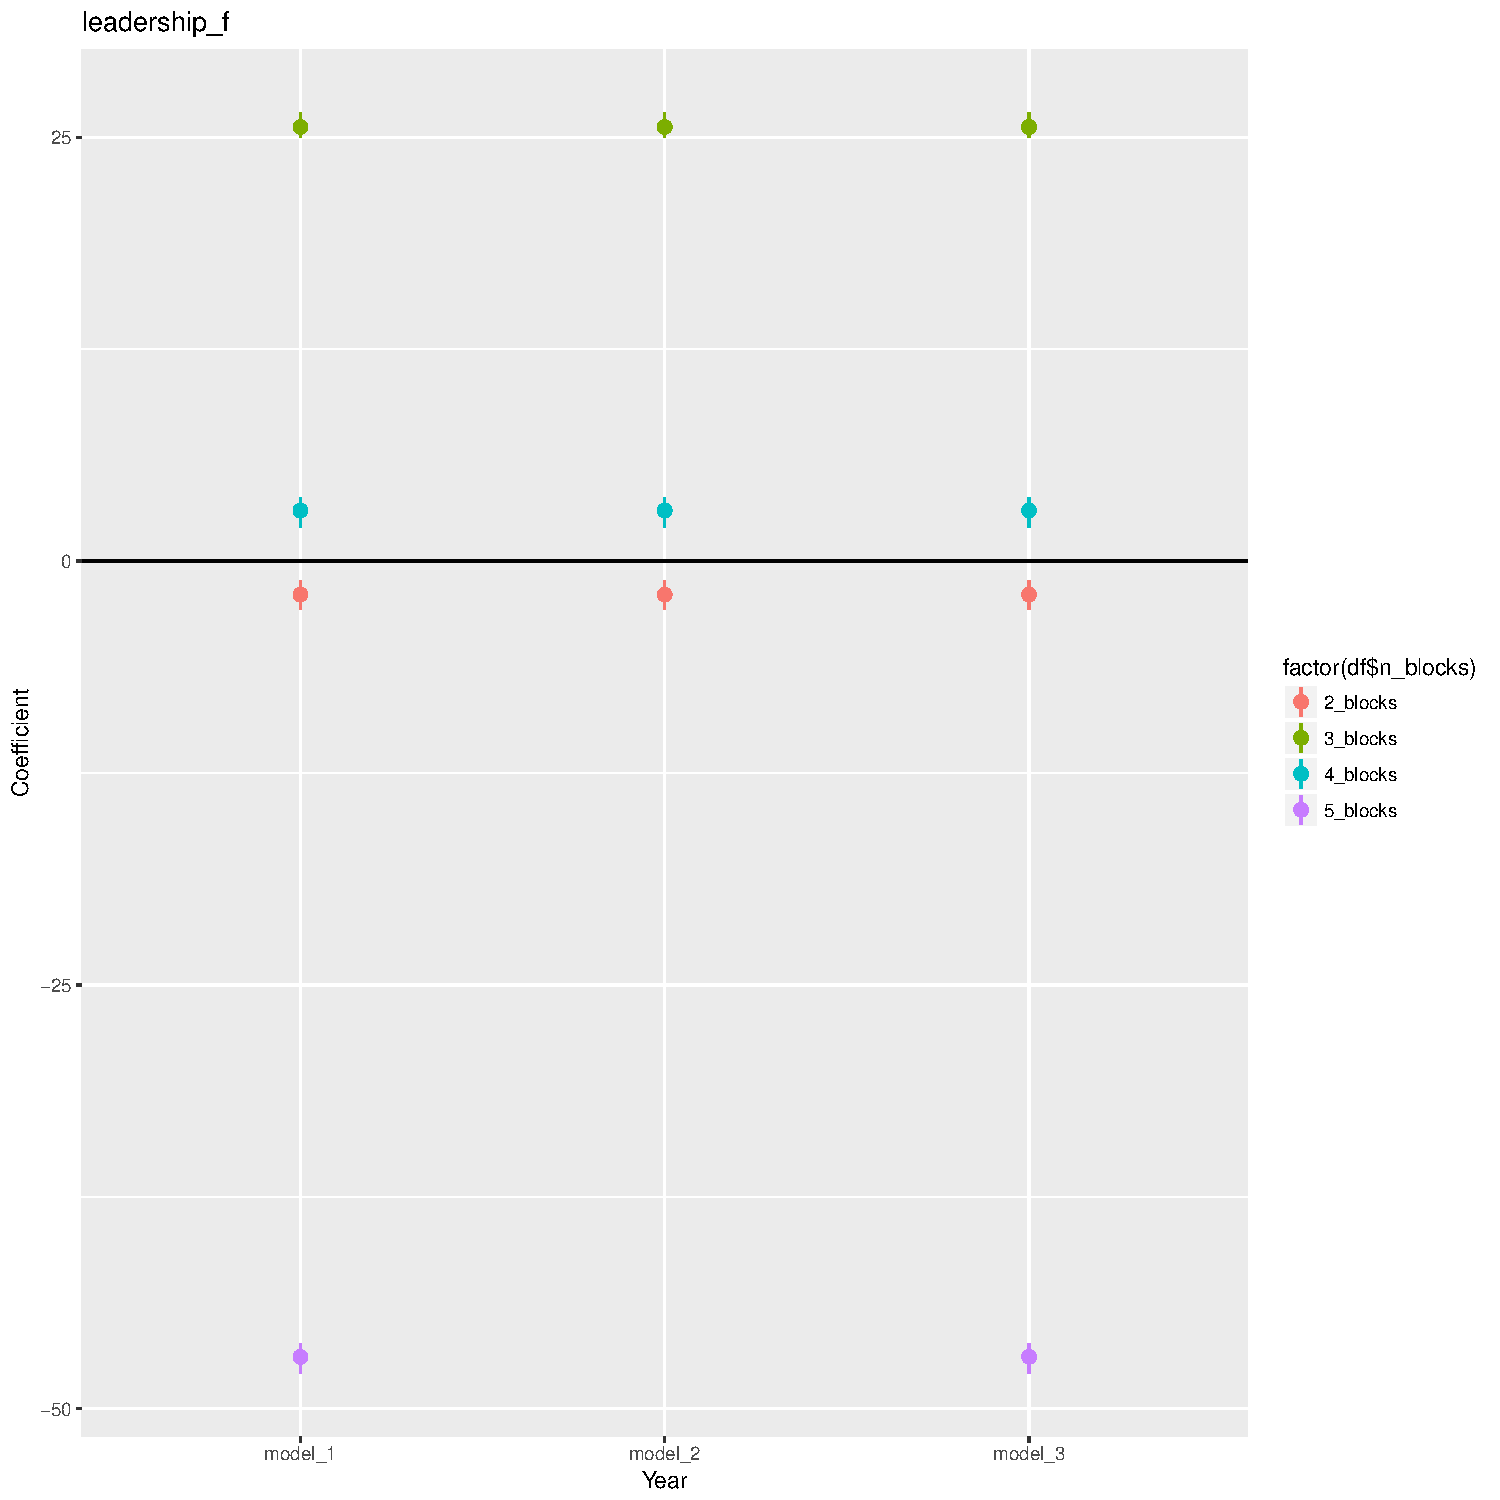
\includegraphics[height=.75\textheight, clip=true, trim=.5cm .5cm 0cm .6cm]{figures/rl_plots1/leadership_f.pdf}   \\
\caption{\label{fig:SBM_plot_com} SBM covariate plot. Results from models for which DIC could not be calculated were discarded.}
\end{longtable}

\clearpage
\begin{longtable}[!h]{c@{\hskip 0cm}c}
In Leadership, nodematch \\
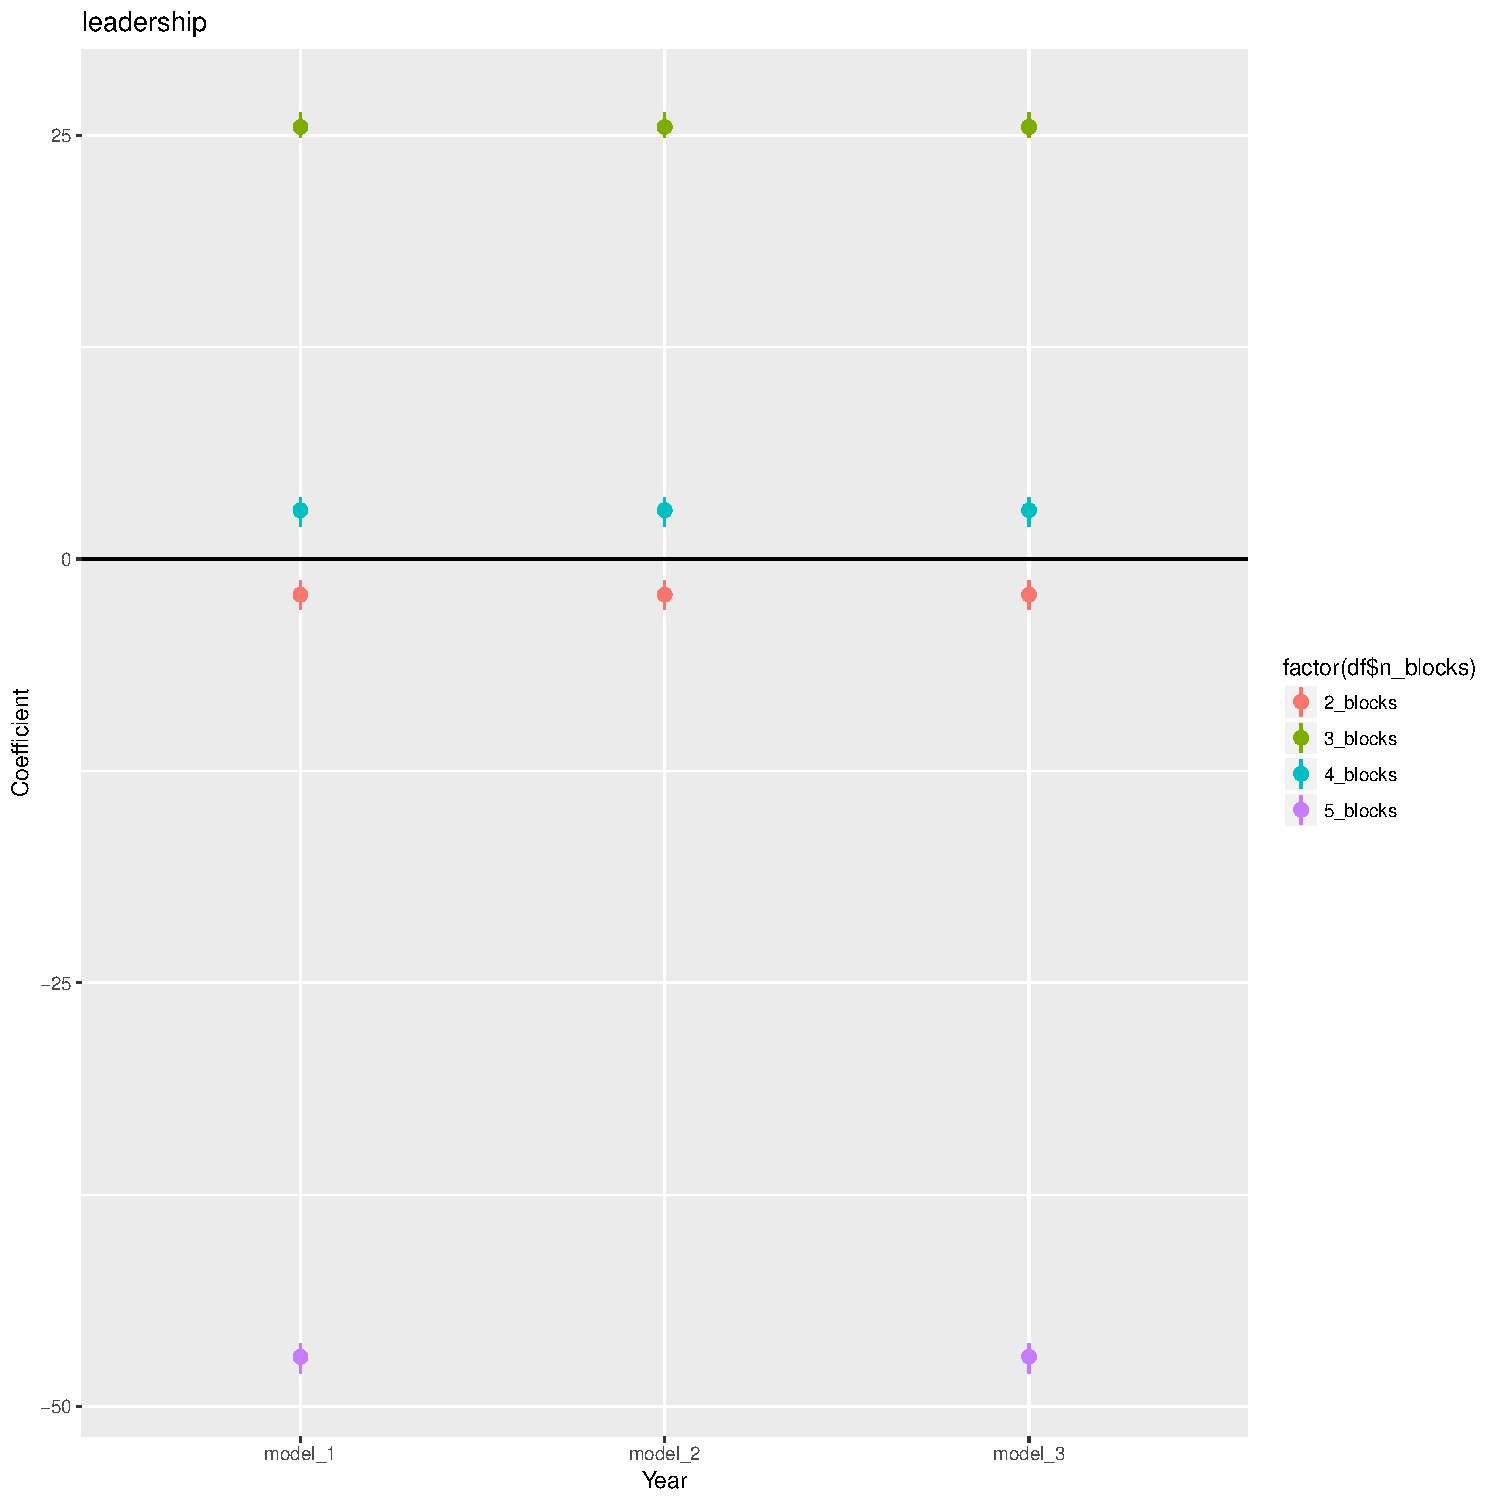
\includegraphics[height=.75\textheight, clip=true, trim=.5cm .5cm 0cm .6cm]{figures/rl_plots1/leadership.pdf}   \\
\caption{\label{fig:SBM_plot_nwsci} SBM covariate plot. Results from models for which DIC could not be calculated were discarded.}
\end{longtable}

\clearpage
\begin{longtable}[!h]{c@{\hskip 0cm}c}
State, nodematch \\
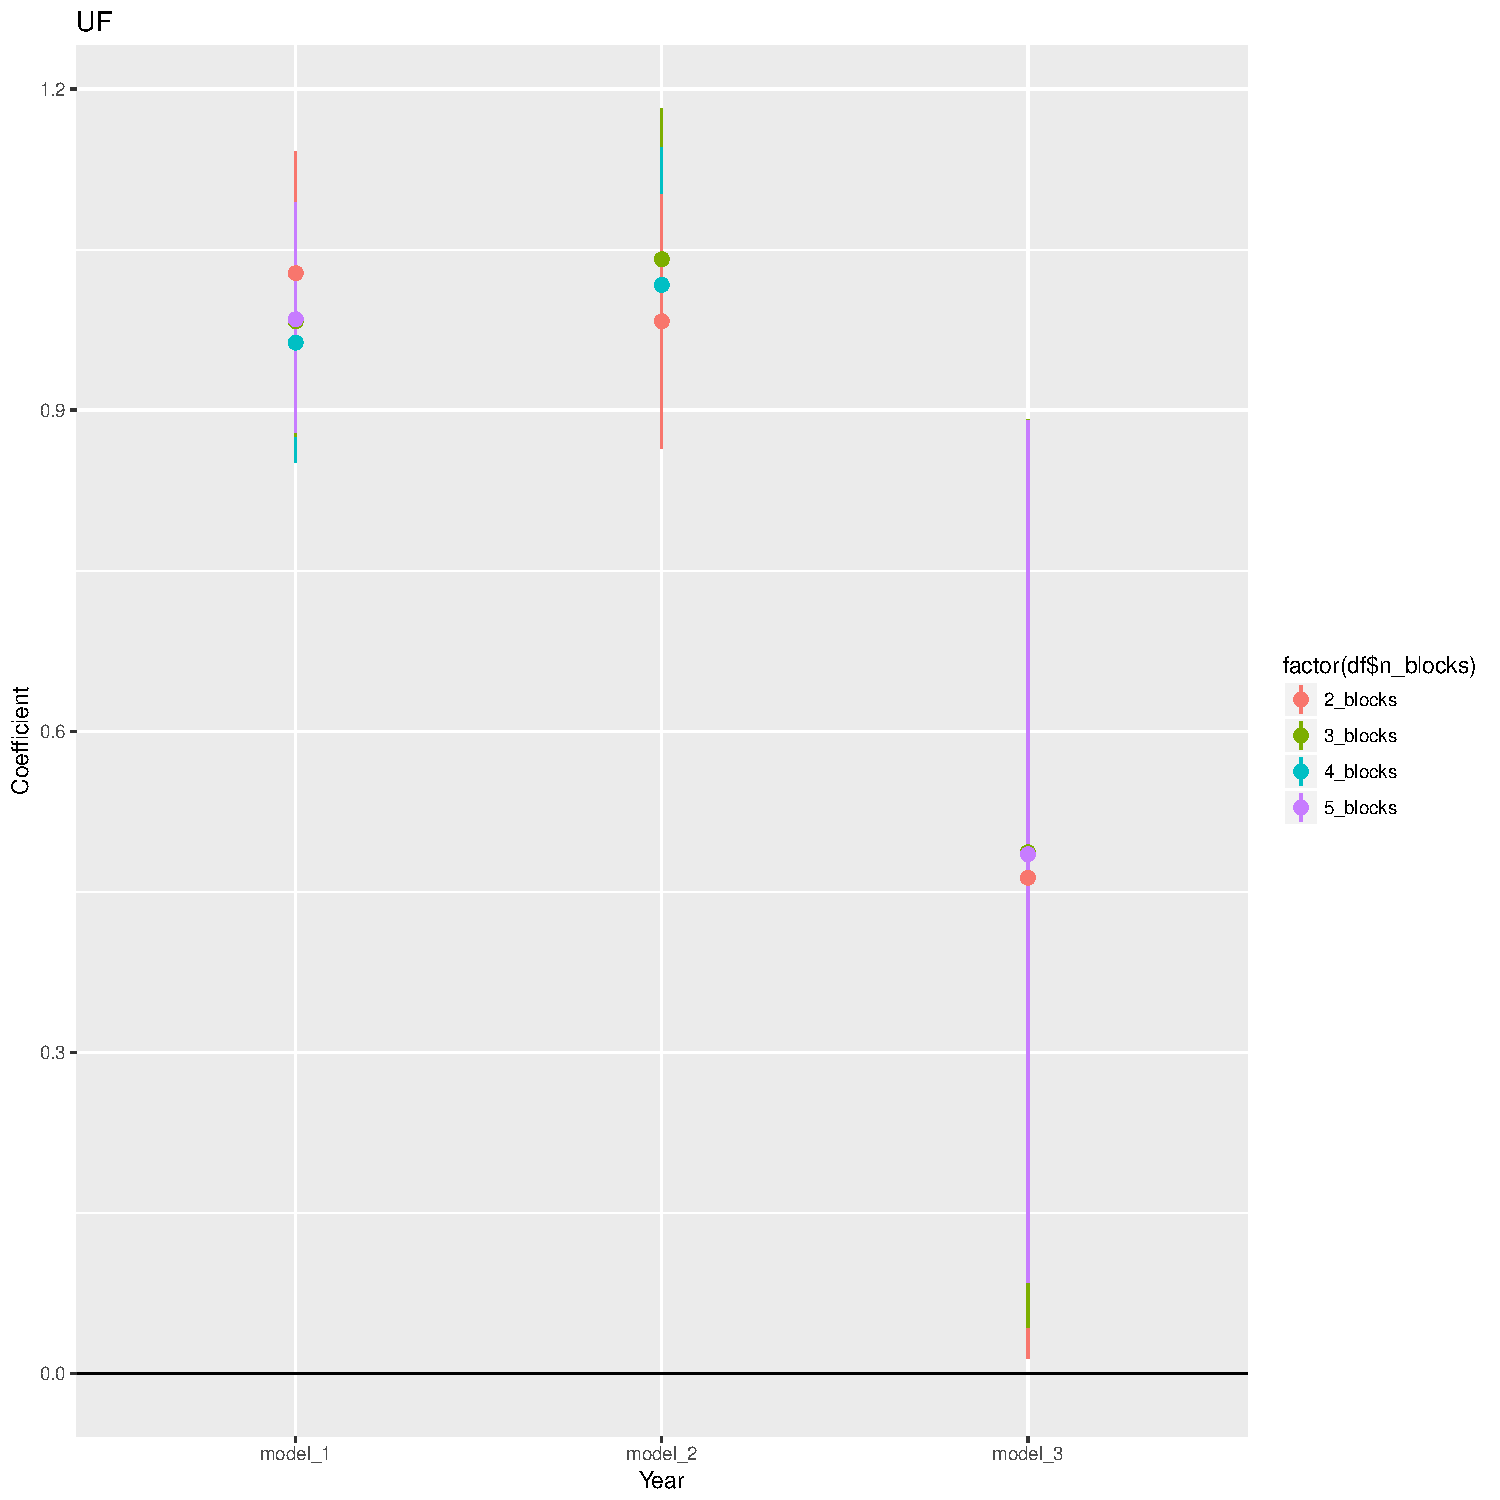
\includegraphics[height=.75\textheight, clip=true, trim=.5cm .5cm 0cm .6cm]{figures/rl_plots1/UF.pdf}   \\
\caption{\label{fig:SBM_plot_nwpol} SBM covariate plot. Results from models for which DIC could not be calculated were discarded.}
\end{longtable}

\clearpage
\begin{longtable}[!h]{c@{\hskip 0cm}c}
Political Party, nodematch \\
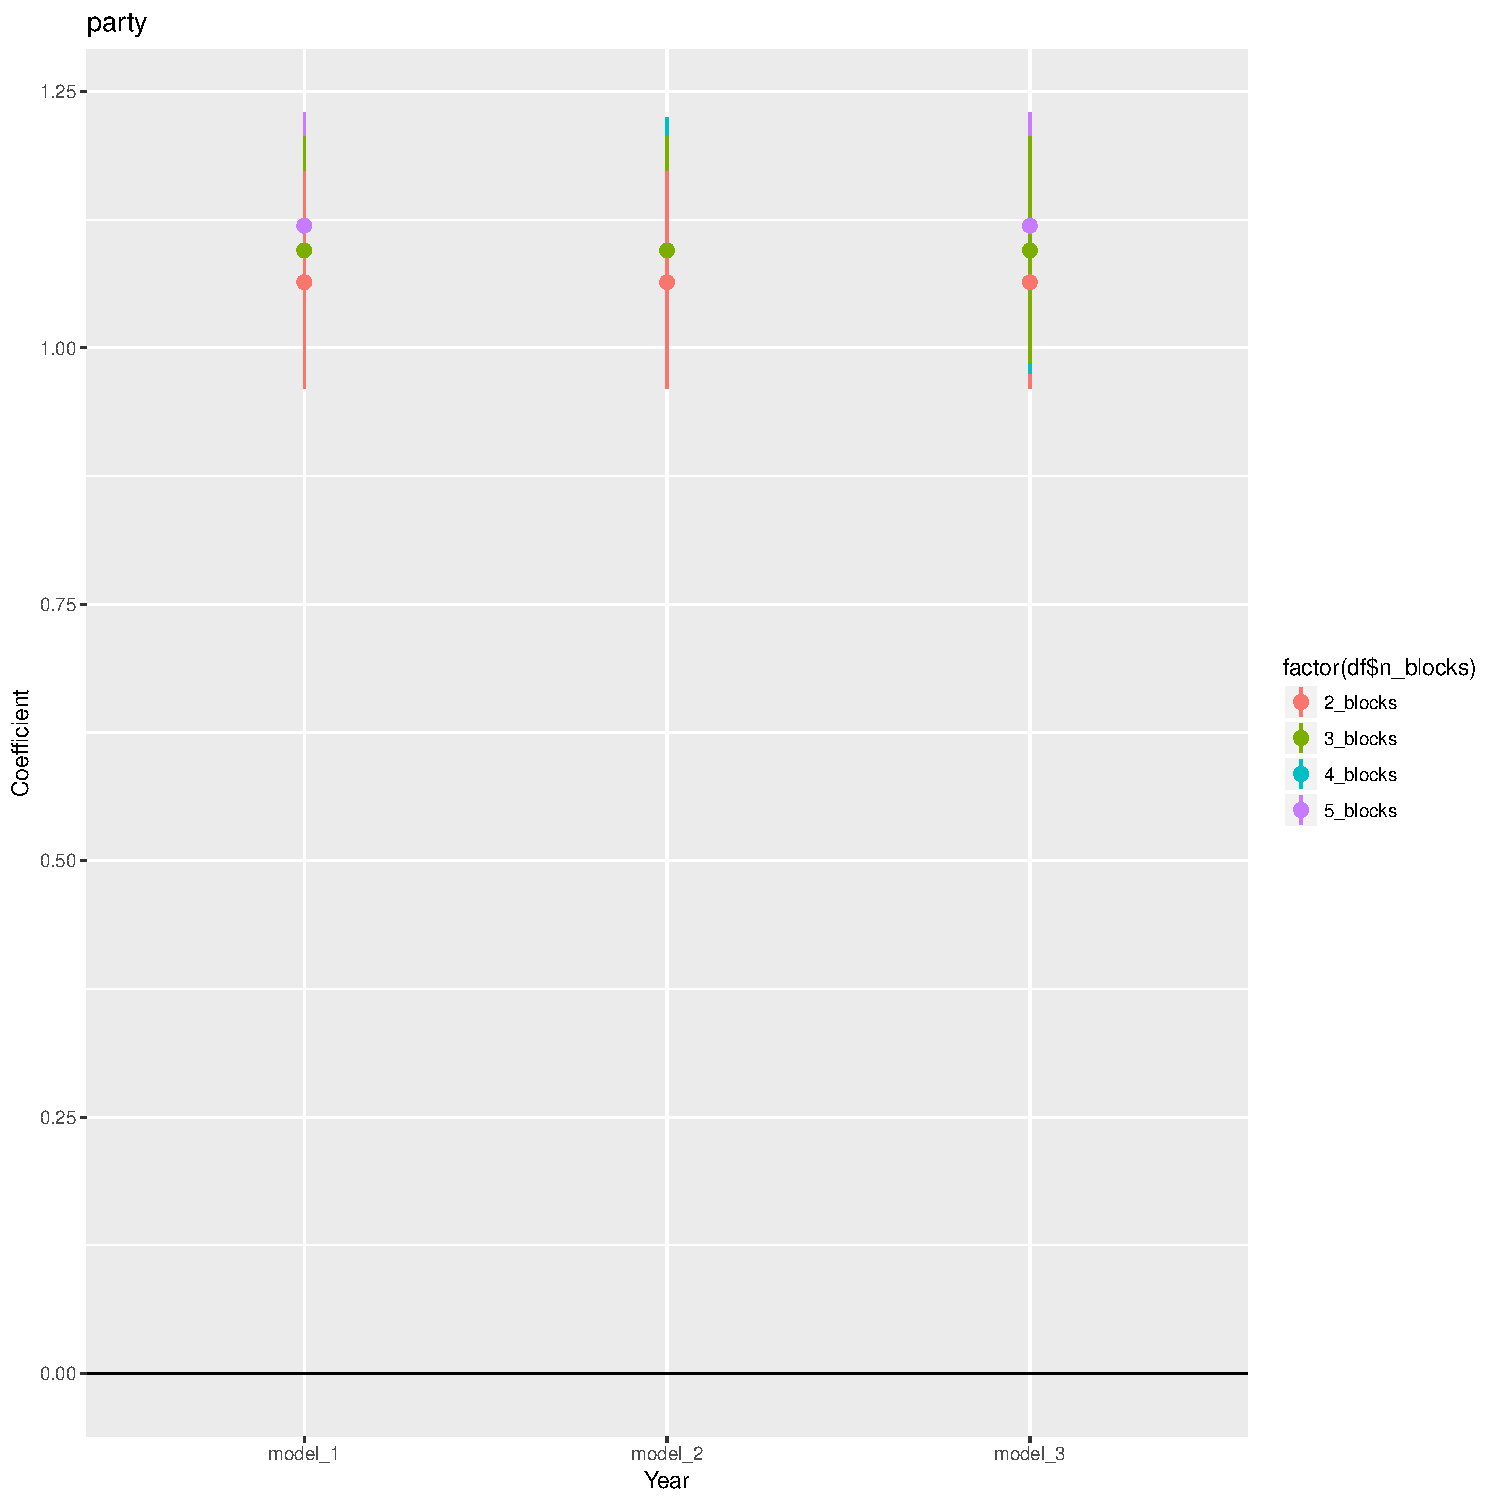
\includegraphics[height=.75\textheight, clip=true, trim=.5cm .5cm 0cm .6cm]{figures/rl_plots1/party.pdf}   \\
\caption{\label{fig:SBM_plot_igig} SBM covariate plot. Results from models for which DIC could not be calculated were discarded.}
\end{longtable}


\bibliographystyle{apsr}
\bibliography{bibliography}




\end{document}